\chapter{Metadata visualizations}\label{layer}

Representing catalog metadata aligned by simulation ID and colored by the Equation of state in the case of BNS systems can be very useful. It can be escalated to any number of parameters. Reading through metadata using them is much easier than dealing with data extraction and unit conversion, in case the developer of the catalog or simulations provides it. 

For instance, inspired by the Core BNS catalog paper, physical metadata can be stacked to know what kind of binary system produced a waveform.


\begin{figure}[hbt!]
\begin{center}
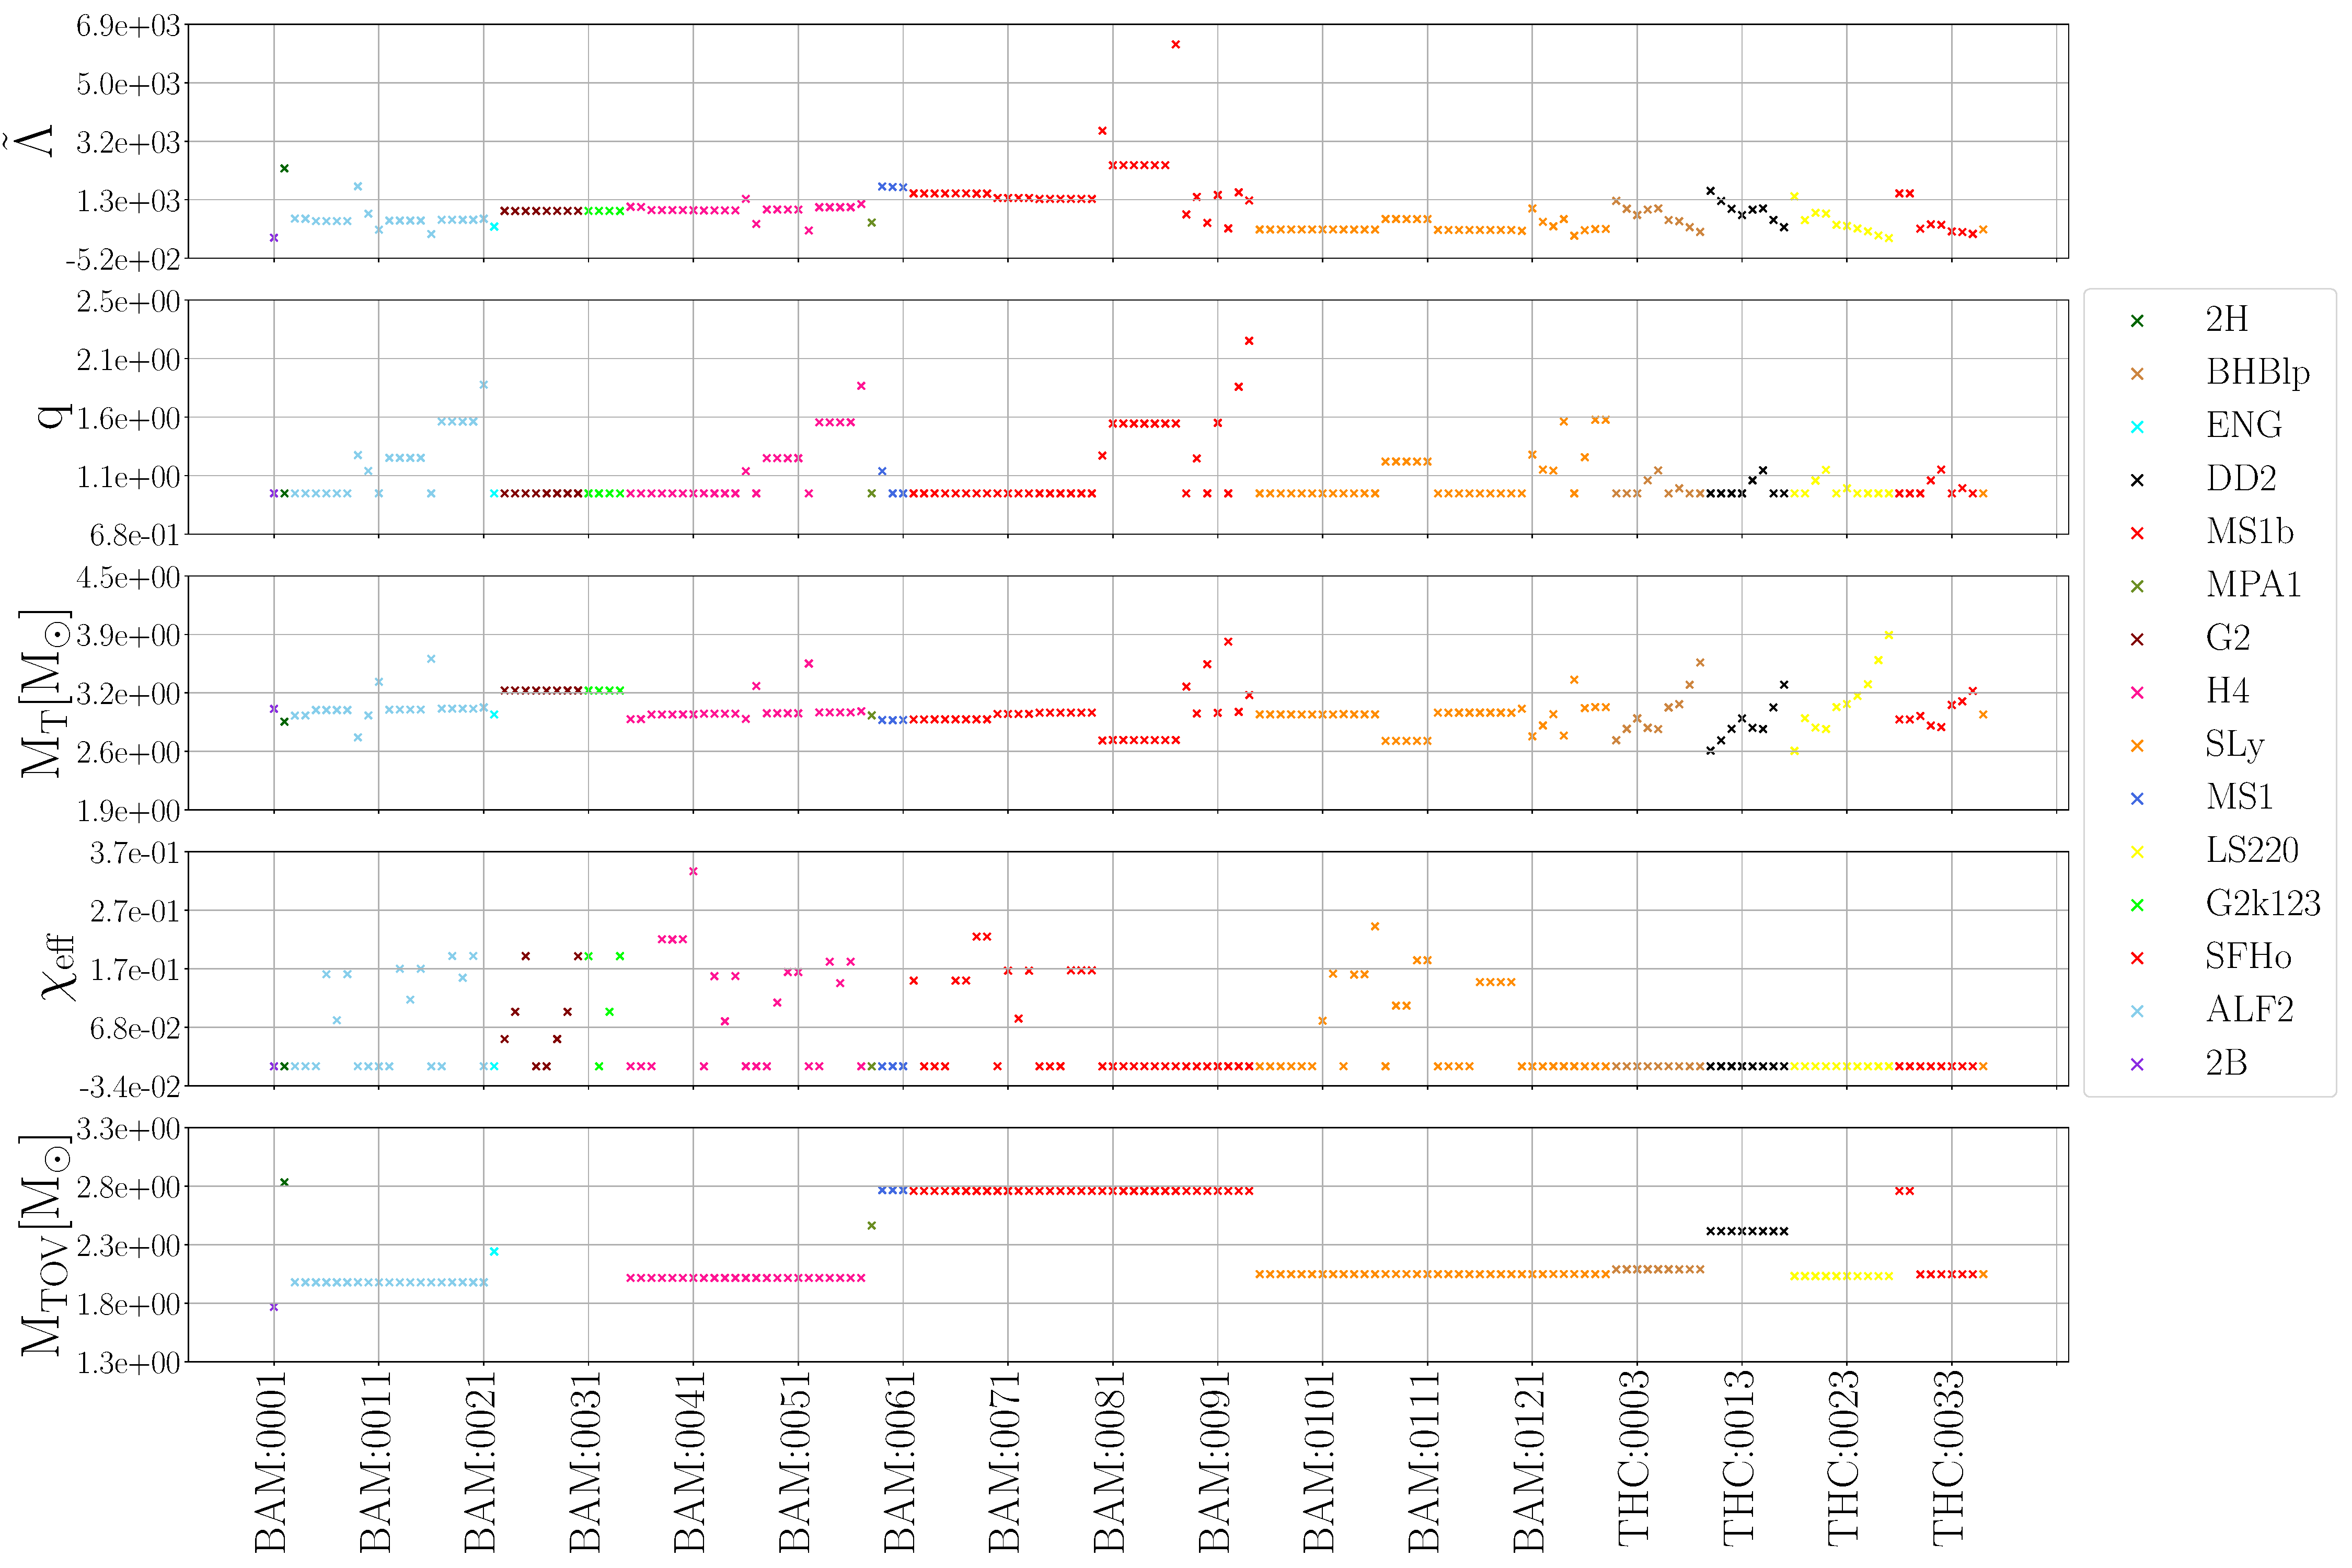
\includegraphics[width=0.9\textwidth, angle=0]{images/Data_analysis/results/CORE_cat.pdf} 
\caption{CoRe BNS catalog metadata}
\end{center}
This image shows a useful way of representing metadata from the simulations. The simulations available in the CoRe catalog\cite{Dietrich:2018phi} provide information about the spins, masses, and tidal deformabilities. Further research had to be done to find the maximum TOV masses for most of the equations of state present in the catalog. Dots are colored according to the Equation of state(right).
\label{corecat}
\end{figure}

\begin{figure}[hbt!]
\begin{center}
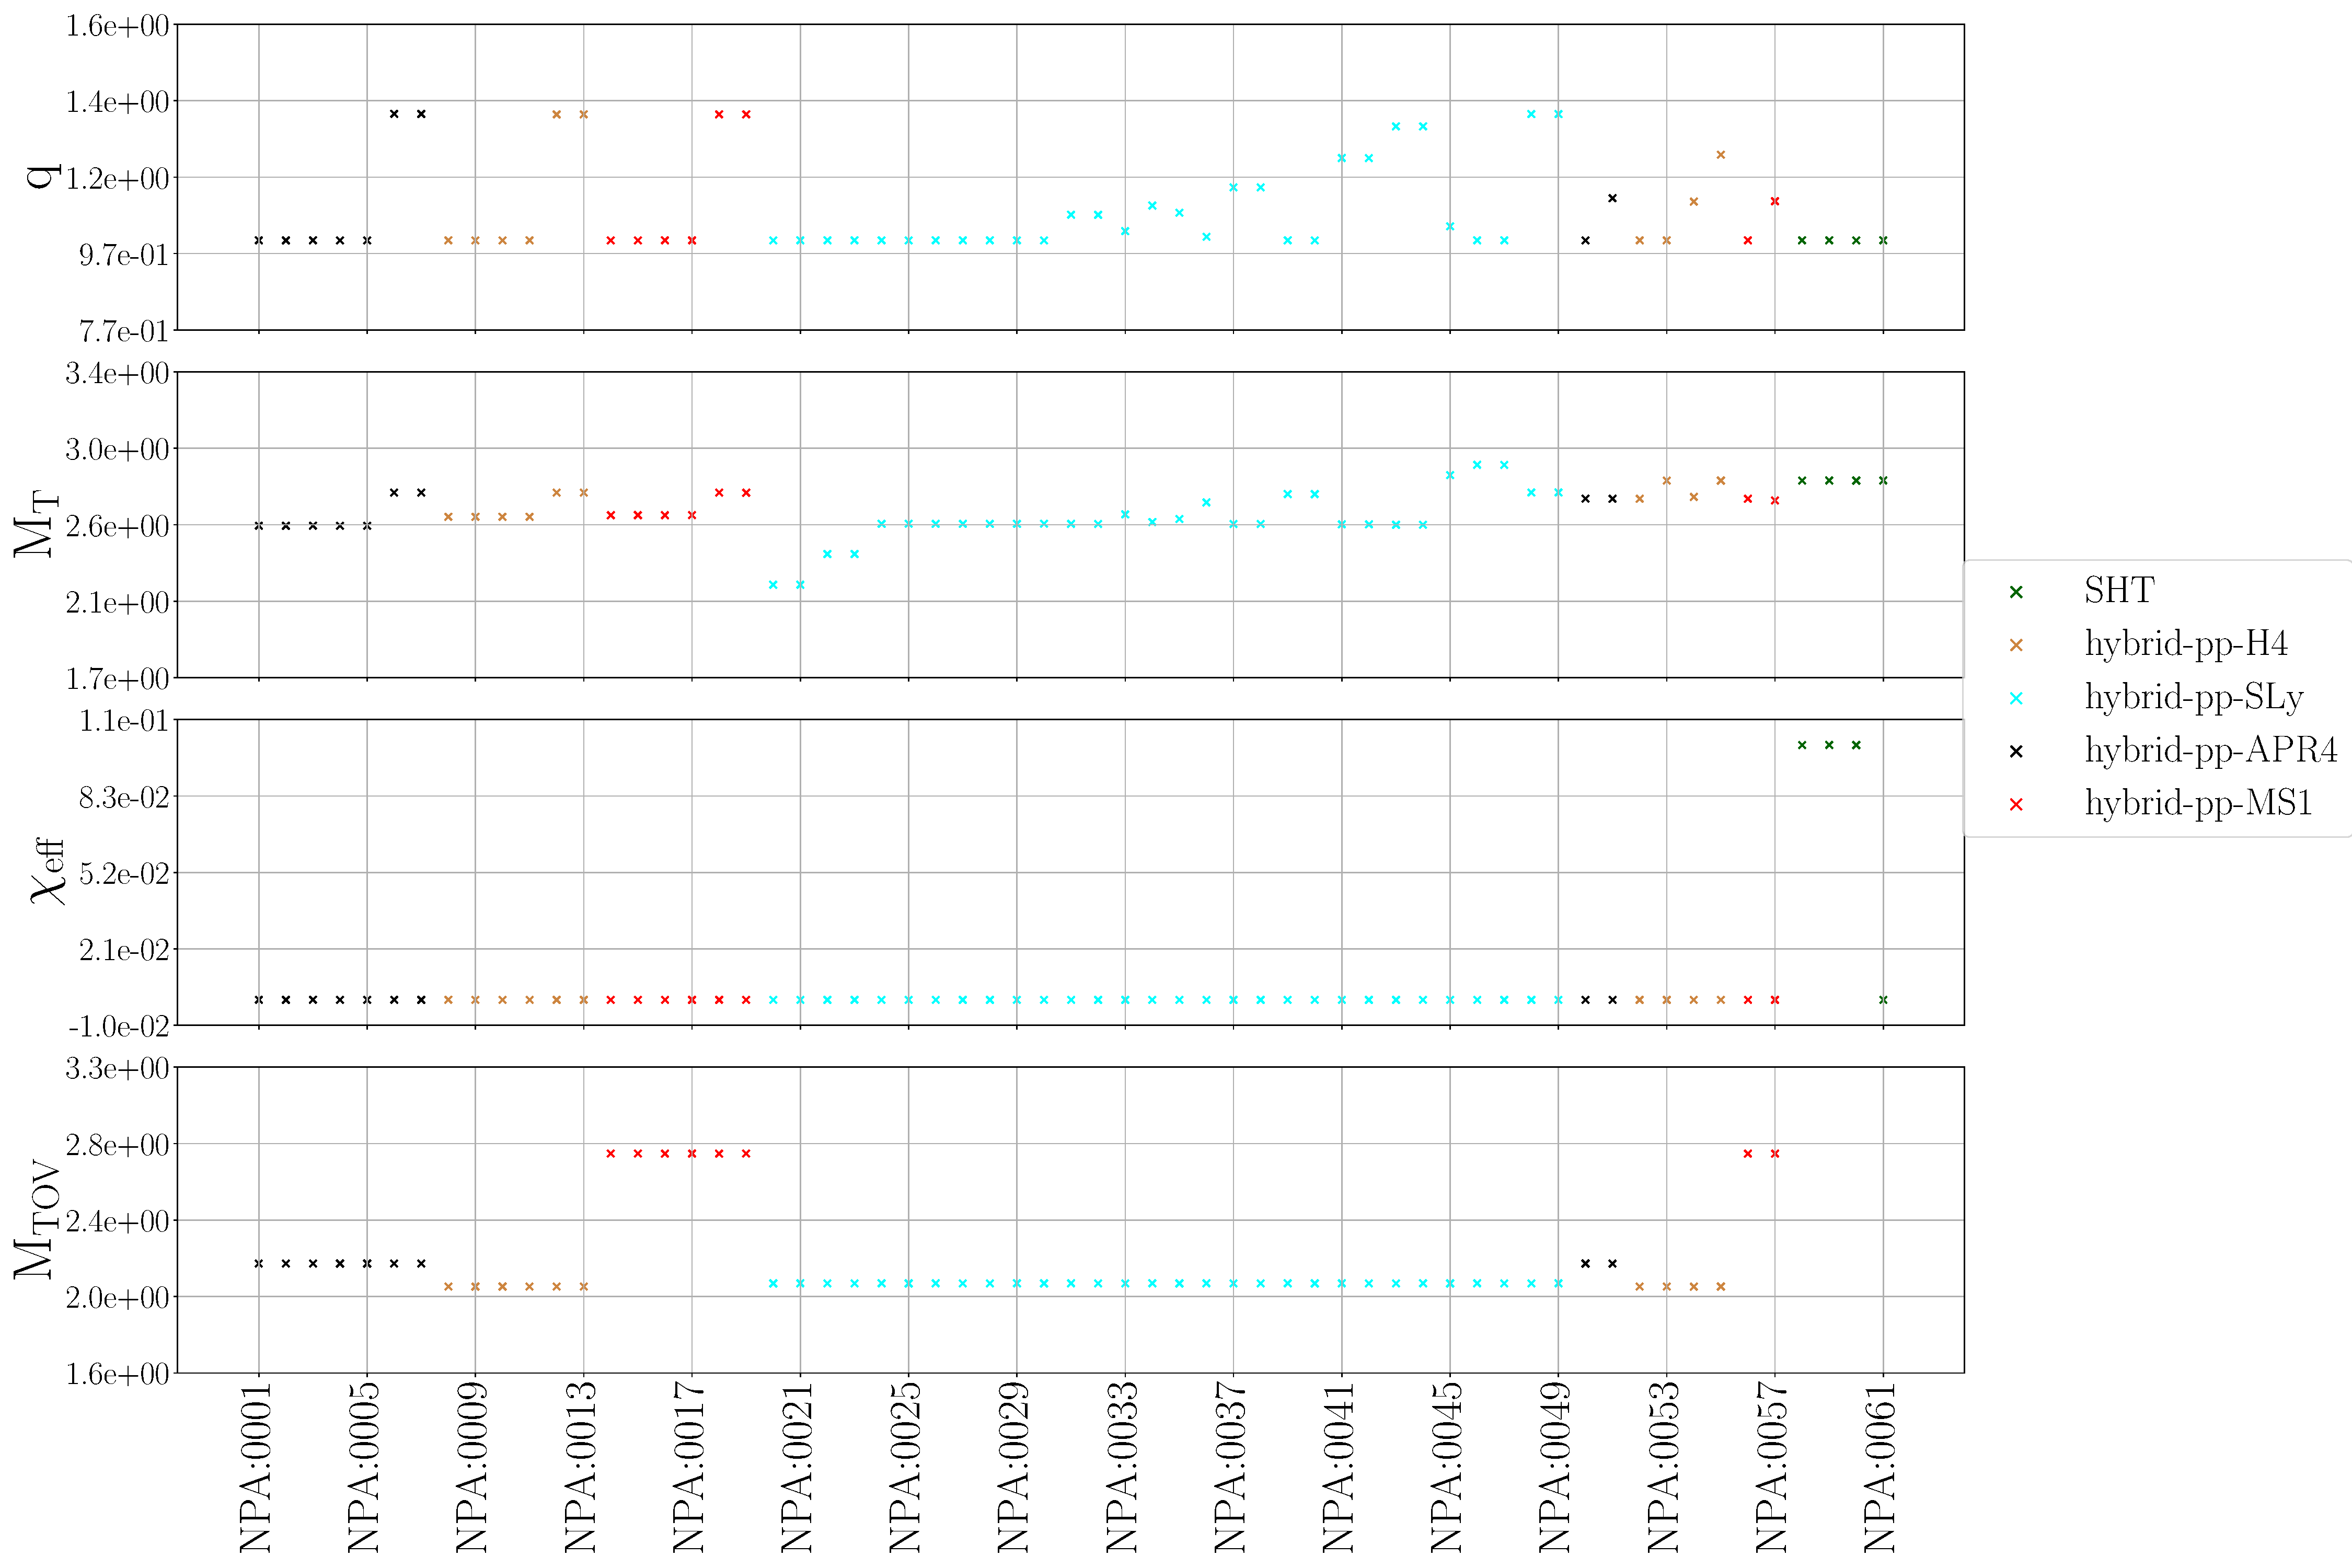
\includegraphics[width=0.9\textwidth, angle=0]{images/Data_analysis/results/LAL_cat.pdf} 
\caption{Metadata coming from other waveforms outside the CoRe catalog}
\end{center}
This image shows a useful way of representing metadata from the simulations. Waveforms represented in this figure came from publicly and non-publicly available data produced by several different authors \cite{Maione:2016zqz, Kastaun:2016elu, Maione:2017aux, Ciolfi:2017uak, Feo:2016cbs, Kawamura:2016nmk, DePietri:2015lya, DePietri:2018tpx}. As one can see, the authors provided masses and spins. However, the tidal deformability was not. Dots are colored according to the Equation of state(right).
\label{lalcat}
\end{figure}

\FloatBarrier


